\documentclass{article}
\usepackage{amsmath,amssymb}
\usepackage{graphicx,color}
\usepackage{gensymb}

\title{\bf{Final Project Report: C++ implementation of the Metropolis-Hasting Algorithm}}
\author{Nicholas Malaya \\ University of Texas at Austin} \date{}

\begin{document}
\maketitle

\section{Introduction}

Bayesian Inference is a powerful statistical method that has found a
variety of applications in uncertainty quantification, decision theory,
model selection and many others. These methods have been applied to
diverse fields such as epidemiology, spam filters, computer vision, as
well as assessments of the reliability of the readiness of the United
States nuclear weapon stockpiles.  

However, Bayes' Theorem, despite existing since the 18th century, has
only recently become more prevalent in scientific applications. The
recent dramatic growth in Bayesian methods coincides with the
exponential expansion of computational power. This is because for all
but a small set of models, the posterior distribution is unable to be
analytically determined, and must be statistically sampled, often
requiring far more samples than are humanly possible to generate. 

For this project, we have developed a C++ implementation of the
Metropolis-Hastings algorithm. This is a Markov Chain Monte Carlo (MCMC)
method to sample from a probability distribution.  These samples will be
generated in order to estimate the posterior of a distribution for a
Bayesian Inference problem. We present results for two distributions, a Gaussian and Beta, 
although it would be very simple to extend this software to other distributions. 

The code is written in C++, and parallelized with openMP. 
\section{Methodology}
%
% 3-4 page report on the progess of the project 
%

Suppose we have a posterior that we want to sample from, but:
\begin{itemize}
 \item the posterior doesn't look like any distribution we know (no
       conjugate model exists)
 \item some (or all) of the full conditionals do not look like any
      distributions we know (no Gibbs sampling) 
\end{itemize}
In these cases, it is necessary to sample the underlying (and often
quite complicated) distribution. The Metropolis-Hastings algorithm
accomplishes this. 

Alternatively, we could sample from the distribution only using ``Vanilla'' 
MC (Monte-Carlo) methods. However, this method unnecessarily discards otherwise useful 
information. As an example, consider figure one below. In this instance, the red dot shows a location
that when sampled, would be rejected because it falls outside of the function's mass. 

\begin{center}
 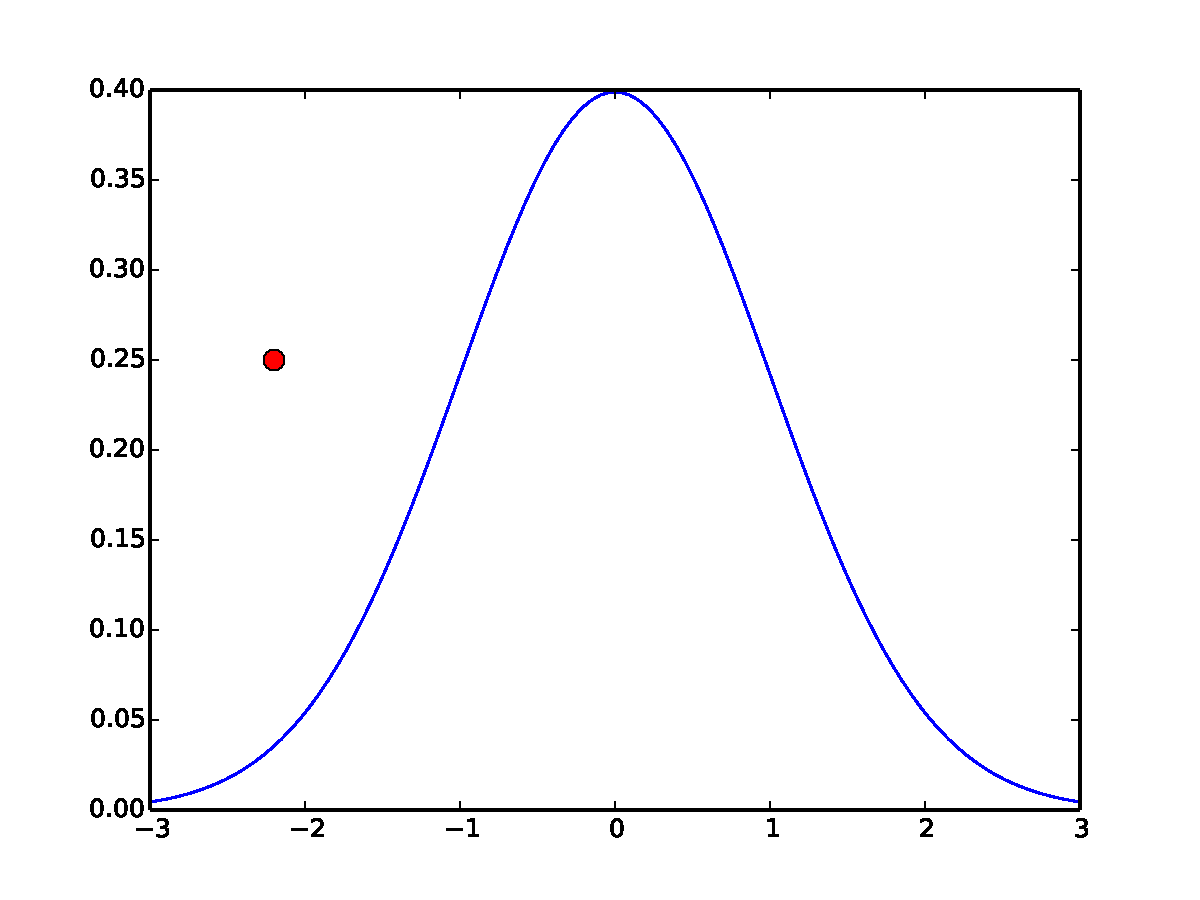
\includegraphics[width=3.5in]{figs/norm}
\end{center}

Next, in figure two, we have another sample that is colored green, and would be accepted in this instance. 
However, instead of again completely randomly sampling a point in the designated interval, 
we should take advantage of the fact that we know this latest point is now within the region we are interested in sampling. 
Thus, instead of simply randomly generating a new sample, we desire to sample a point that is ``nearby'' the latest one. In this way, 
each point we sample is correlated with the last step we made. When each step only depends on the last step, 
this is known as a ``Markov Process''. 

\begin{center}
 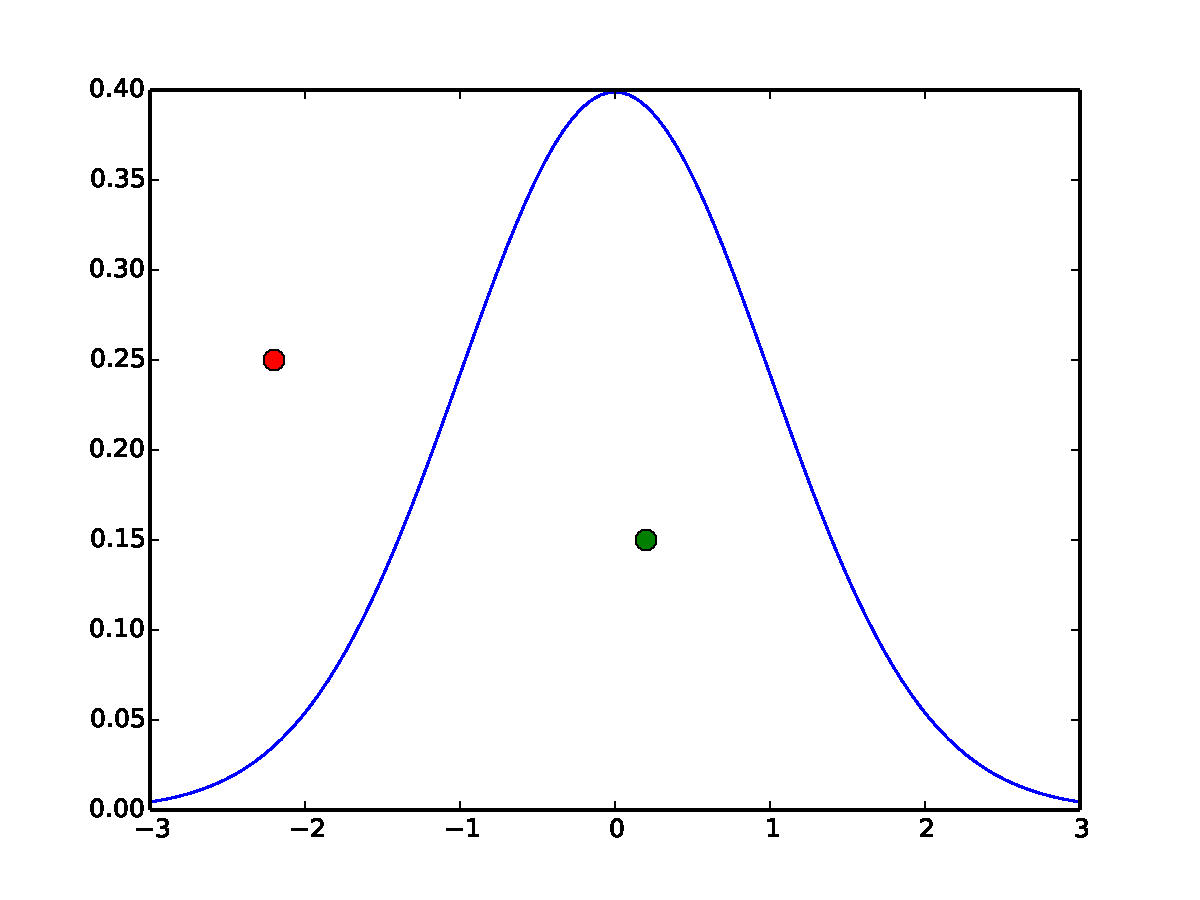
\includegraphics[width=3.5in]{figs/norm-acc}
\end{center}

Figure three shows such a guess. Here, we have colored blue around a region adjacent to the latest guess. 
By restricting our guess to a local region near the latest accepted chain, we hope to more efficiently (but still stochastically!) 
sample the integral. There are many different ways we might ``propose'' a location near the last accepted sample. This decision, as well as 
a more detailed discussion of the particular MCMC algorithm we are implementing, are discussed in the next section. 

\begin{center}
 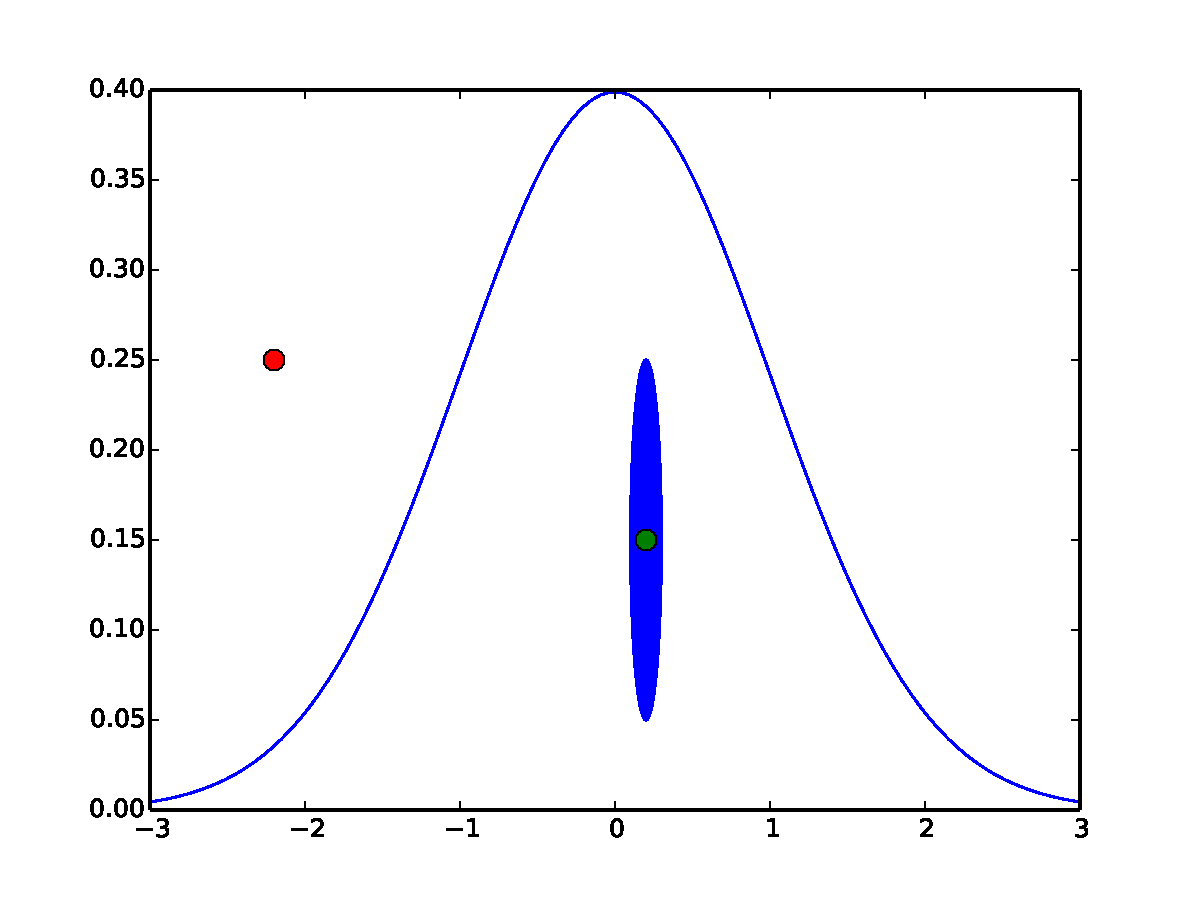
\includegraphics[width=3.5in]{figs/norm-corr}
\end{center}

\subsection{Model Document: The Metropolis Hastings Algorithm}

The Metropolis-Hastings Algorithm is an MCMC algorithm for generating samples. There are many ways we might 
``guess'' out next point around the last one. Metropolis-Hastings ``proposes'' a location nearby randomly, by drawing random samples 
from a specified probability density function. 

For each Metropolis step, we begin with a guess for the starting point,
$\phi_1$. Afterward, we begin sampling. Each step of this so-called,
``rejection sampling'' involves ``proposing'' a new value, which if it
meets a specified criterion, is accepted. The next step then begins. 

Thus, we begin with a proposal step (in this case, for step two),
\begin{equation}
 q(\tilde \phi_2 | \phi_1) = N(\tilde \phi_2 | \phi_1, \nu^2).
\end{equation}
In other words, our proposal step is correlated with the previous step,
in that it is drawn from a Gaussian (Normal) distribution with mean of
the previous step, and standard deviation, $\nu$. We will discuss our
choice of $\nu$ more, later. In order to draw this proposal, we generate a 
proposal from a standard normal distribution, Z, and then transform it according to,
\begin{equation}
 X = \phi_1 + \nu*Z.
\end{equation}

Thus, with our new proposal $\tilde \phi_2$ drawn, we must evaluate
whether to accept this or reject it. In order to accomplish this, we
next draw from a uniform distribution, $u \sim U(0,1)$. 

Now, we accept the new $\tilde \phi_2$ if it meets the following
criterion, 
\begin{equation}
u < \frac{\pi_n(\tilde \phi_2)}{\pi_n(\phi_1)}. 
\end{equation}
If we accept, then $\tilde \phi_2$ becomes $\phi_2$, and we begin the
next step. If we reject, then we keep our present value, e.g. $\phi_2 = \phi_1$. 

Now as we proceed, you might ask, what dictates whether we accept or
reject? Well, after the ``burn-in'' period, where we move around looking
for the region where the distribution has non-zero probability, we
eventually start sampling the posterior. Here, we want to ``jump''
around in each guess just enough that we will capture the tails of the
distribution, but simultaneously, we don't want to jump so far that we
move away from the areas of the distribution that has most of the
probability associated with it. This is where our $\nu$ comes in. This
is the variance of the proposal. If it is very large, then we will tend
to make large jumps away from the mean for our proposal. These are great
for finding the distribution in the first place, and they will tend to
capture more of the tails, but simultaneously, too many large jumps will
result in more rejections by our sampling algorithm. Therefore, we need
to balance $\nu$ so that is jumps around, but not too far.

It turns out that mathematicians have shown that for various situations,
an, ``acceptance ratio'' of right around 40\% is just about right. This
acceptance ratio is simply the ratio of accepted proposals to total MCMC
steps we have taken. Therefore, we have tried to tune our $\nu$
parameter for each situation to have an acceptance ratio around 40\%. 

Note that while we chose for this project a Gaussian distribution, this is not
a required feature. One could use nearly any other sort of proposal distribution. A gaussian
has several appealing features, namely, it is easily generalized to multi-dimensions, it is inexpensive to 
compute, and it is a smooth function.  One other very useful feature of a Gaussian is that the 
proposal distribution is symmetric, that is to say,
\begin{equation}
  f(x) = f(-x). 
\end{equation}
This might not seem particularly important, but it actually significantly simplifies the sampling algorithm above. 
Furthermore, note that just because the proposal distribution is not symmetric does not mean that this particular 
algorithm cannot sample non-symmetric distributions. In the results section later in this report 
we will successfully sample the Beta distribution (which is non-symmetric), despite using a proposal distribution
that is symmetric. However, a non-symmetric proposal distribution might be more effective at sampling such a 
distribution. 

\section{Using the Library}

The metropolis algorithm as detailed above has now been implemented in a few hundred lines of C++. 
The codebase for this project has been developed on bitbucket, with logs
 for each commit. A fully functioning build system (a makefile) alongside a 'make  
 check' regression suite has been developed. At present, three
 regression tests are run, that perform simple checks on the distributions and sampling algorithm. 
The code has been tested on a local i7 quad core laptop, as well as TACC's lonestar supercomputer. 

Finally, a directory, ``postprocessing'' contains scripts used to
generate all plots. These are routines using python with numpy+scipy and
matplotlib. 

The library should be run as follows:

\begin{itemize}
\item make
\item make check (this runs a series of tests
\item make install (installs your routines to a local bin/)
\item make run (executes the c++ metropolis-hastings routines)
\item cd ../postproc
\item python hist-gauss.py (to generate a histogram from the gaussian sampling)
\item python hist-beta.py (to generate a histogram from the beta sampling)
\item inspect hist-gauss.png and hist-beta.png
\end{itemize}

\section{Results}

Figure four shows a histogram of the samples from a Gaussian distribution. 
Shown are $1e5$ steps which are used to verify that our distribution matches a known posterior. 
\begin{center}
 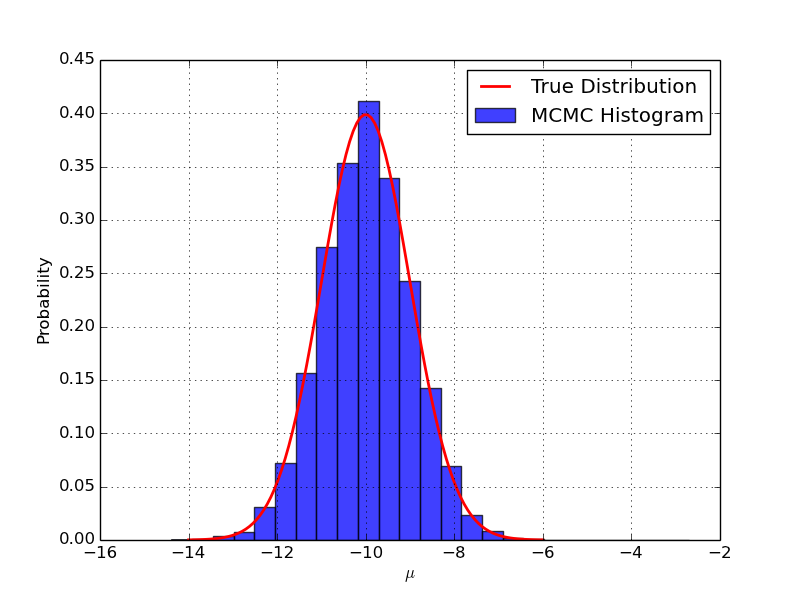
\includegraphics[width=3.5in]{figs/hist-gauss}
\end{center}

Likewise, Figure five shows a histogram of the samples from a $\beta$ distribution. 
Shown are $1e5$ steps which are used to verify that our distribution matches this posterior. 

\begin{center}
 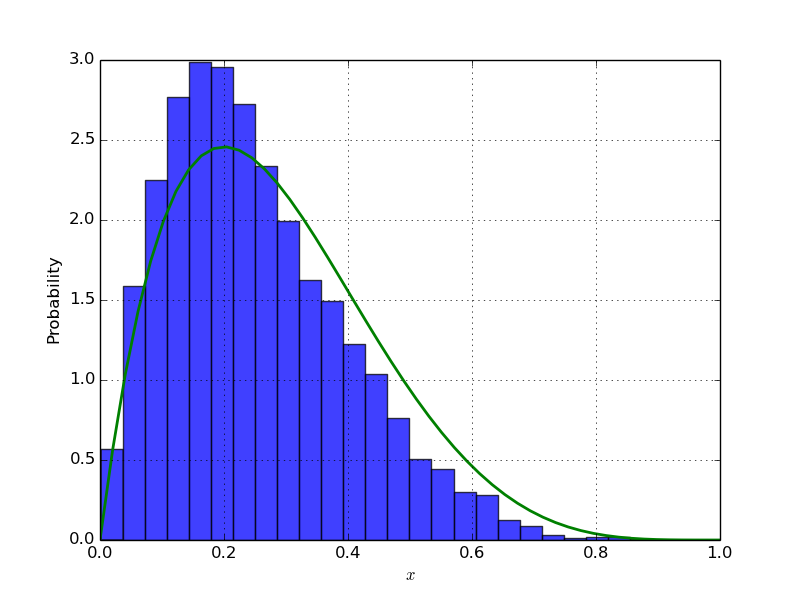
\includegraphics[width=3.5in]{figs/hist-beta}
\end{center}

Now you might say, this doesn't fit particularly well! And you are somewhat correct. 
The mean seems to be over-predicted (higher than the green line) and the tail (off near $x=1$) is under-resolved. 
This is not too surprising, as it is harder to resolve the tails, and generally takes more samples. This image looks very much like 
a not-converged set of samples! So let's bump up the number of samples to $1e7$ to see if things match more closely. This is show in figure six, below.

\begin{center}
  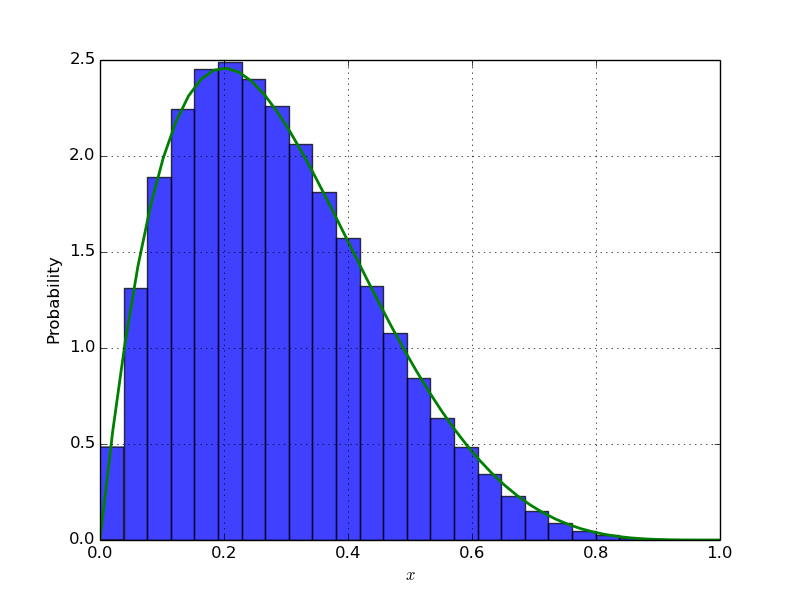
\includegraphics[width=3.5in]{figs/hist-beta_10e7}
\end{center}

Much better. We have now resolved the tail and the mean matches the result much more closely! So why am I showing you this, instead of 
just starting with $1e7$ and showing you those results? Because it is an example of how MCMC can be tricky: without that exact result 
(which we typically do not have, or we would have no reason to use MCMC!) we would not have known that we had too few samples. So one must be careful to ensure that
the system is ``converged'', in particular, that the mean, standard deviation, shape of the histogram, etc. are all not changing as a function of the number of steps. 

\section{OpenMP Multithreading}

In MCMC, one can also instantiate multiple chains, which advance for each 
Markov-chain step based on the same algorithm as outlined above. In other words, 

Each chain is completely independent, and the parallel problem is ``embarrassingly parallel'', e.g. we 
do not require any communication between chains during the runs. This means we anticipate near-perfect scalability. 

In order to accomplish this, we start each chain at a slightly different location, by perturbing each chain 
slightly from our initial guess. Then, each thread can run completely independently, and at the end of the run, 
we will combine the chains together. 

Preparing this in the code is relatively straight-forward. We have created a third driver routine, entitled, ``metropolis-omp'' that is created at compile time when using the command, ``make''. This routine is compiled with the C++ compiler, adding only, 

\begin{itemize}
\item -fopenmp -lpthread
\end{itemize}
for GCC, or for intel:

\begin{itemize}
\item -openmp
\end{itemize}

to the \$LDFLAGS variable. A standard C++ compiler (such as intel's icpc or GNU's G++) will then enable OpenMP. 
At this point, we create as many chains as there are threads, using the omp\_get\_max\_threads() method. We can also
vary the number of threads by calling the omp\_set\_num\_threads(n) method, where n here is the desired number of threads.
Each chain is given a number of steps to run, which are appended to a file. This is all parallelized 
using a PRAGMA, in particular, ``\#pragma omp for'' before the loop that runs each chain. 
At this point, each chain can run indepdendently. 

The plot of the strong scaling is shown below. Regrettably, very little speedup is seen. This is because the computation is relatively modest, 
and the vast majority of the computation appears to be in File I/O as well as spawning the threads. Therefore,
the advantage of multiple threads is completely mitigated. 

\begin{center}
  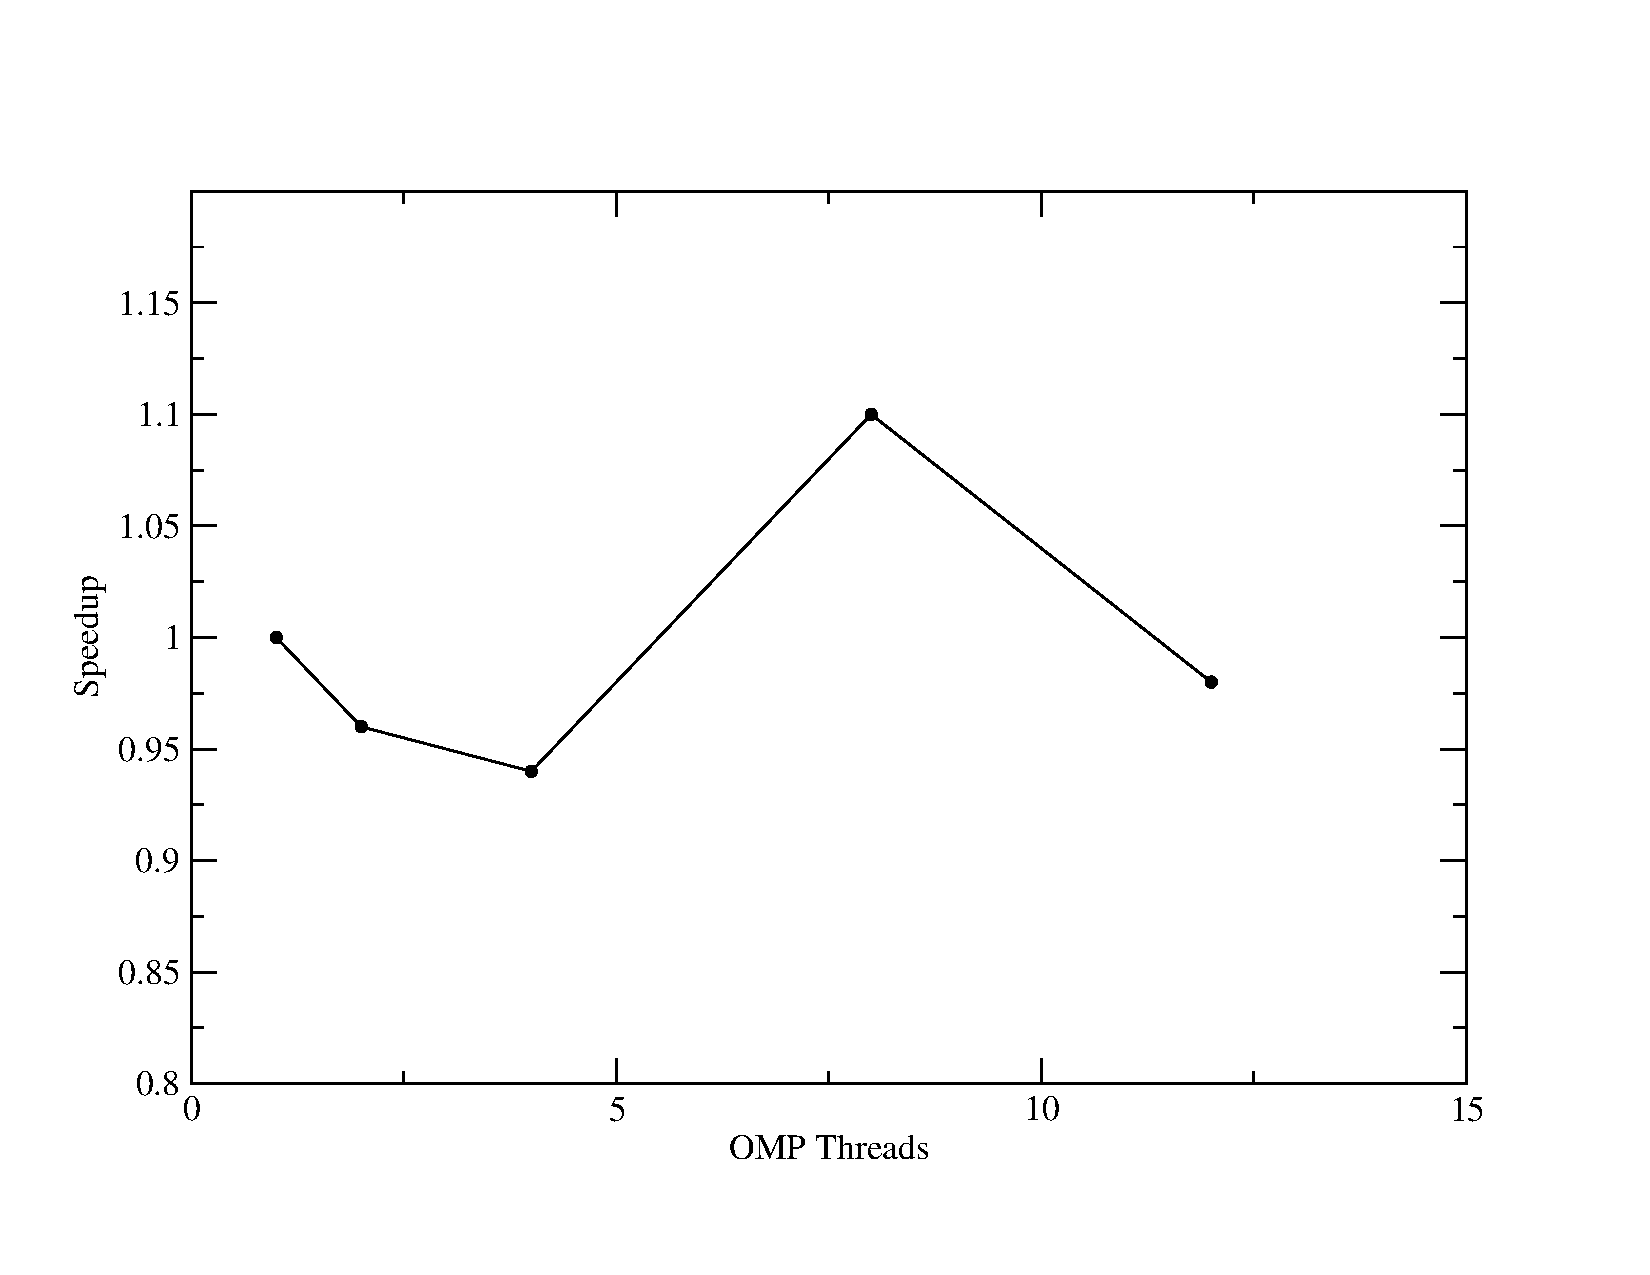
\includegraphics[width=3.5in]{figs/data}
\end{center}


We could likely fix this by changing how the code runs: presently, at each step of the sampler, the present
MCMC chain location is written to disk. It would be far more efficient to capture all the samples
in an array, and then after each thread has finished sampling, and then writing that entire array to disk. 

\section{Conclusions}

We have shown how to formulate an MCMC rejection sampler, the Metropolis-Hastings algorithm. For this we use a gaussian distribution for the proposal. We have instantiated a C++ implementation 
of this algorithm, which we have tested for the Gaussian and Beta distributions. Finally, we developed an OpenMP parallelization around this algorithm. 

All the code is available in project/src. The postprocessing used to generate the plots are stored in project/postproc. Finally, this entire report, the figures and the LaTeX used to generate this PDF 
are all stored in project/final. 

I had fun writing a Metropolis-Hastings sampler, which is a very fundamental algorithm in computational 
statistics. Thank you for reading this document and examining the project. I'm sure this is an involved and time-consuming process. Thank you for the class, and have a happy Holiday Season!

--Nicholas Malaya

\end{document}
